
\medskip  

\parbox{0.4\linewidth}{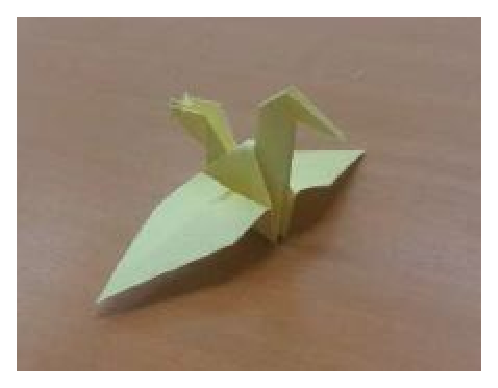
\includegraphics[width=0.3\textwidth]{grue.eps}}\hfill
\parbox{0.6\linewidth}{
L'\textbf{origami} est le nom japonais de l'art du pliage du papier. À partir d'un carré de 15 cm, on donne ci-dessous le début du canevas de pli de la grue japonaise.}

\bigskip

\parbox{0.38\linewidth}{\psset{unit=1cm}
\begin{pspicture*}(-2.5,-3)(2.5,2.5)
%\psgrid
\psline[linestyle=dotted](-2.5,0)(2.5,0)
\psline[linestyle=dotted](0,-2.5)(0,2.5)
\psline[linestyle=dotted](-2.5,-2.5)(2.5,2.5)
\psline[linestyle=dotted](-2.5,2.5)(2.5,-2.5)
\psframe(-2.5,-2.5)(2.5,2.5)
\psline[linestyle=dashed](-2.5,-2.5)(0,3.536)(2.5,-2.5)
\psline[linestyle=dashed](-2.5,2.5)(3.536,0)(-2.5,-2.5)
\psline[linestyle=dashed](2.5,-2.5)(-3.536,0)(2.5,2.5)
\psline[linestyle=dashed](-2.5,2.5)(-0.42,-2.5)
\psline[linestyle=dashed](0.42,-2.5)(2.5,2.5)
\pspolygon(0,1.46)(1.04,1.04)(1.46,0)(1.04,-1.04)(0,-1.46)(-1.04,-1.04)(-1.46,0)(-1.04,1.04)
\uput[ur](0,1.46){A} \uput[ur](1.04,1.04){B} \uput[ur](1.46,0){C} 
\uput[r](1.04,-1.04){D} \uput[dr](0,-1.46){E} \uput[d](-1.04,-1.04){F} 
\uput[dl](-1.46,0){G} \uput[l](-1.04,1.04){H} \uput[dr](0,0){O}
\uput[d](0,-2.5){\footnotesize Cette figure n'est pas en vraie grandeur}
\end{pspicture*}
}\hfill 
\parbox{0.6\linewidth}{
\begin{enumerate}
\item Cette construction fait apparaitre un polygone régulier ABCDEFGH de centre O. Est-ce un pentagone, un octogone ou un hexagone? 
\item Calculer alors la mesure de l'angle $\widehat{\text{AOB}}$. 
\item Calculer ensuite la mesure de l'angle $\widehat{\text{OAB}}$. 
\item On donne OA = OC = 4,5 cm. Calculer la longueur AC. Arrondir au dixième. 
\end{enumerate}}

\vspace{0,5cm}

